\documentclass[../../main.tex]{subfiles}
\graphicspath{{../../image/}{../../figure/}}
\begin{document}

\section{熵率容许性准则}\label{section:ch09-熵率容许性准则}

按熵激波容许准则,跨激波的熵产生(由\eqref{align:ch08-熵条件}左端定义)必须为负,特别地总熵须递减。然而我们已经看到,此要求一般判别力不足,无法排除一切赝解。这里将引入一种波扇容许准则,它是熵容许条件的强化版本:它规定波扇中所有激波的组合熵产生不只是负的,而且要尽可能小;等价地,正如事实所表明的,总熵不只是递减,而是以最高容许速率递减。

假定方程组\eqref{align:ch09-9-1-1}配有指定的熵-熵流对 $(\eta(U),q(U))$,并考虑端状态为 $V(-\infty)=U_{L}$、$V(\infty)=U_{R}$ 的波扇 $U(x,t)=V(x/t)$ 的容许性。$V$ 中各激波的组合熵产生为
\begin{align}
\mathscr{P}_{V}=\sum_{\xi}\bigl\{q(V(\xi+))-q(V(\xi-))-\xi[\eta(V(\xi+))-\eta(V(\xi-))]\bigr\},
\label{align:ch09-9-7-1}
\end{align}
其中求和遍历 $V$ 的至多可数个跳跃间断点 $\xi$ 集。

由于 Rankine-Hugoniot 跳跃条件\eqref{align:ch09-9-1-8},对任一 $\Theta\in\mathbb{M}^{1\times n}$ 与 $a\in\mathbb{R}$,熵-熵流对 $(\eta(U)+\Theta U+a,\ q(U)+\Theta F(U))$ 给出与 $(\eta(U),q(U))$ 相同的组合熵产生。因而不妨不失一般性地假定
\begin{align}
\eta(U_{L})=\eta(U_{R})=0.
\label{align:ch09-9-7-2}
\end{align}

在此规范化之后,波扇中总熵的变化率为
\begin{align}
\dot{\mathscr{H}}_{V}=\frac{\mathrm{d}}{\mathrm{d}t}\int_{-\infty}^{\infty}\eta(U(x,t))\,\mathrm{d}x
=\frac{\mathrm{d}}{\mathrm{d}t}\int_{-\infty}^{\infty}\eta\!\left(V\!\left(\frac{x}{t}\right)\right)\mathrm{d}x
=\int_{-\infty}^{\infty}\eta(V(\xi))\,\mathrm{d}\xi.
\label{align:ch09-9-7-3}
\end{align}

事实上, $\mathscr{P}_{V}$ 与 $\dot{\mathscr{H}}_{V}$ 由
\begin{align}
\dot{\mathscr{H}}_{V}=\mathscr{P}_{V}+q(U_{L})-q(U_{R})
\label{align:ch09-9-7-4}
\end{align}
联系。为验证此式,从恒等式
\begin{align}
\eta(V(\xi))=[\xi\eta(V(\xi))-q(V(\xi))]^{\cdot}+\dot{q}(V(\xi))-\xi\dot{\eta}(V(\xi)),
\label{align:ch09-9-7-5}
\end{align}
(它在测度意义下成立)出发,并注意广义链规则(\cref{theorem:ch01-Gauss-Green})给出
\begin{align}
\dot{q}(V)-\xi\dot{\eta}(V)=[\widetilde{\mathrm{D}q}(V)-\xi\widetilde{\mathrm{D}\eta}(V)]\dot{V}.
\label{align:ch09-9-7-6}
\end{align}
由\eqref{align:ch09-9-7-6}、\eqref{align:ch07-熵流对定义}与\eqref{align:ch09-9-1-6}推知,测度 $\dot{q}(V)-\xi\dot{\eta}(V)$ 集中在 $V$ 的跳跃间断点集上。因而合并\eqref{align:ch09-9-7-1}、\eqref{align:ch09-9-7-2}、\eqref{align:ch09-9-7-3}与\eqref{align:ch09-9-7-5},即得\eqref{align:ch09-9-7-4}。

\begin{definition}[熵率容许性准则]\label{definition:ch09-熵率容许性准则}
波扇 $U(x,t)=V(x/t)$,其中 $V(-\infty)=U_{L}$、$V(\infty)=U_{R}$,满足\emph{熵率容许性准则},若对任一端状态同为 $\bar{V}(-\infty)=U_{L}$、$\bar{V}(\infty)=U_{R}$ 的其他波扇 $\bar{U}(x,t)=\bar{V}(x/t)$,有 $\mathscr{P}_{V}\leqslant\mathscr{P}_{\bar{V}}$,或等价地 $\dot{\mathscr{H}}_{V}\leqslant\dot{\mathscr{H}}_{\bar{V}}$。
\end{definition}

联系连续介质物理,熵率容许准则是热力学第二定律的一个更强版本:物理熵不仅应增加,而且应以质量、动量、能量平衡律所容许的最大速率增加。动理论似乎为这一论旨提供了某种佐证,至少对小振幅波如此(文献见\cref{section:ch09-注记})。然而熵率原理的地位最终须依据它在熟悉方程组中的推论以及它与其他确立已久的容许条件的比较来评判。这正是我们接下来的任务。

我们先在标量守恒律上检验熵率准则。此时波扇由单个(一般为复合)波组成。

\begin{theorem}\label{theorem:ch09-标量熵率}
对标量守恒律\eqref{align:ch07-标量守恒律},一个波扇对任意指定的严格凸熵 $\eta$ 满足熵率准则,当且仅当每个激波满足 Oleinik $E$ 条件\eqref{align:ch08-oleinik}。
\end{theorem}

\begin{proof}
为简单起见,我们把证明限于单向波扇类,尽管结论在无此限制时也成立。令 $u(x,t)=v(x/t)$ 为\eqref{align:ch07-标量守恒律}的任一单向波扇,端状态 $u_{L}$、$u_{R}$ 给定。不妨设 $u_{L}<u_{R}$(相反情形 $u_{L}>u_{R}$ 类似),则 $v$ 是 $(-\infty,\infty)$ 上的非减函数,满足微分方程
\begin{align}
[f(v(\xi))-\xi v(\xi)]^{\cdot}+v(\xi)=0,\qquad-\infty<\xi<\infty,
\label{align:ch09-9-7-7}
\end{align}
边值 $v(-\infty)=u_{L}$、$v(\infty)=u_{R}$。

我们把 $v$ 延拓为极大单调多值函数 $\tilde{v}$:在 $v$ 的任一跳跃间断点 $\xi$ 处,把区间 $[v(\xi-),v(\xi+)]$ 取为 $\tilde{v}$ 的值。然后取 $\tilde{v}$ 的(极大单调)逆函数 $\xi$,并令
\begin{align}
h(u)=f(u_{L})+\int_{u_{L}}^{u}\xi(v)\,\mathrm{d}v,\qquad u_{L}\leqslant u\leqslant u_{R}.
\label{align:ch09-9-7-8}
\end{align}

注意 $h$ 是 $[u_{L},u_{R}]$ 上的凸函数, $h(u_{L})=f(u_{L})$, $h(u_{R})=f(u_{R})$。此外,对任一 $u\in(u_{L},u_{R})$,要么 $h(u)=f(u)$,要么 $h(u)\neq f(u)$ 且
\begin{align}
h(u)=\frac{(u_{+}-u)f(u_{-})+(u-u_{-})f(u_{+})}{u_{+}-u_{-}},
\label{align:ch09-9-7-9}
\end{align}
其中 $u_{L}\leqslant u_{-}<u_{+}\leqslant u_{R}$。因而,如\cref{figure:ch09-标量熵率}所示, $h$ 的图像是 $f$ 图像弧(对应 $v$ 的稀疏波)与 $f$ 图像弦(对应 $v$ 的激波)的拼接。此外, $v$ 的常值状态对应 $h'$ 的跳跃间断点。特别地,由\cref{section:ch09-一般严格双曲方程组}构造、激波满足 Oleinik $E$ 条件的唯一波扇所诱导的 $h$,正是 $f$ 在 $[u_{L},u_{R}]$ 上的下凸包,即\cref{figure:ch09-标量复合波}与\cref{figure:ch09-标量熵率}中描绘的函数 $g$。反之, $[u_{L},u_{R}]$ 上任一具上述性质的凸函数 $h$ 都生成\eqref{align:ch07-标量守恒律}的一个端点为 $u_{L}$、$u_{R}$ 的波扇 $v$。

\begin{figure}[ht]
\centering
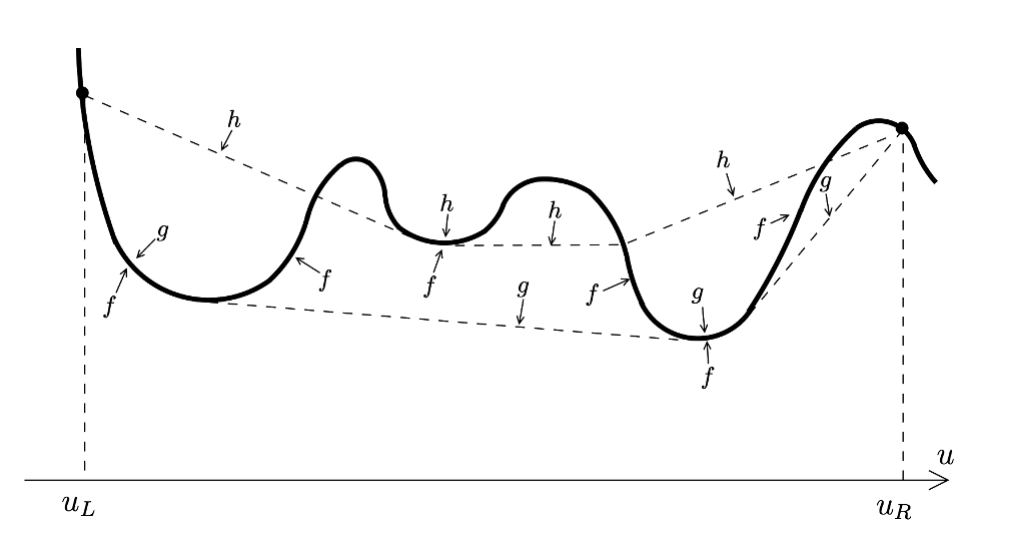
\includegraphics[width=0.85\textwidth]{ch09-fig07-01.png}
\caption{$f$(实线)、凸包 $h$(点线)、下凸包 $g$(虚线);弦长 $h$ 对应激波,弧对应稀疏波。}
\label{figure:ch09-标量熵率}
\end{figure}

现指定某凸熵函数 $\eta$,其相伴流 $q$ 满足 $q'(u)=\eta'(u)f'(u)$,并通过\eqref{align:ch09-9-7-1}计算 $v$ 中激波的熵产生:
\begin{align}
P_{v}&=\sum_{\text{激波}}\{q(v(\xi+))-q(v(\xi-))-\xi[\eta(v(\xi+))-\eta(v(\xi-))]\}
\nonumber\\
&=\int_{u_{L}}^{u_{R}}[q'(v)-h'(v)\eta'(v)]\,\mathrm{d}v
=\int_{u_{L}}^{u_{R}}[f'(v)-h'(v)]\eta'(v)\,\mathrm{d}v
=\int_{u_{L}}^{u_{R}}[h(v)-f(v)]\eta''(v)\,\mathrm{d}v.
\label{align:ch09-9-7-10}
\end{align}
由于对 $v\in[u_{L},u_{R}]$ 有 $h(v)\geqslant g(v)$,故 $P_{v}$ 在 $h=g$ 时最小,即 $v$ 是\cref{section:ch09-一般严格双曲方程组}构造的、激波满足 Oleinik $E$ 条件的唯一波扇。证明完毕。
\end{proof}

现转到一般严格双曲方程组,但把研究限于小振幅激波:

\begin{theorem}\label{theorem:ch09-熵率蕴含liu}
对任一带指定熵-熵流对 $(\eta,q)$ 的严格双曲守恒律方程组\eqref{align:ch09-9-1-1},其中 $\eta$ 局部一致凸,一个具中等强度波的波扇满足熵率容许准则,仅当每个激波都满足 Liu $E$ 条件。
\end{theorem}

\begin{proof}
我们用反证法证明定理断言:给定任一含某个违反 Liu $E$ 条件激波的波扇,我们构造一个熵率更低的波扇。为用最少的技术细节传达论证本质,我们完整讨论波扇由单个激波组成的特殊情形,然后简述一般情形如何处理。

于是设状态 $U_{L}$ 与 $U_{R}$, $|U_{R}-U_{L}|=\delta$, $\delta$ 正且小,由一个速度为 $s$ 的 $i$-激波连接,
\begin{align}
F(U_{R})-F(U_{L})=s[U_{R}-U_{L}],
\label{align:ch09-9-7-11}
\end{align}
该激波违反 Liu $E$ 条件。在规范化\eqref{align:ch09-9-7-2}下,此激波的熵率为零。目标是构造一个同端状态 $U_{L}$、$U_{R}$ 的波扇 $V$,使 $\dot{\mathscr{H}}_{V}<0$。

令 $U_{R}=W_{i}(\tau_{R};U_{L})$。不妨设 $\tau_{R}>0$。由于 Liu $E$ 条件被违反,集 $\{\tau\in(0,\tau_{R}):s_{i}(\tau;U_{L})<s\}$ 非空。令 $\tau_{L}$ 为该集的下确界,并设 $\tau_{L}>0$($\tau_{L}=0$ 的情形更简单)。于是 $s_{i}(\tau_{L};U_{L})=s$,且 $s_{i}(\tau;U_{L})$ 在 $\tau_{L}$ 处递减。我们考虑通有情形 $\dot{s}_{i}(\tau_{L};U_{L})<0$。

置 $U_{M}=W_{i}(\tau_{L};U_{L})$,
\begin{align}
F(U_{M})-F(U_{L})=s[U_{M}-U_{L}].
\label{align:ch09-9-7-12}
\end{align}
合并\eqref{align:ch09-9-7-11}与\eqref{align:ch09-9-7-12},
\begin{align}
F(U_{R})-F(U_{M})=s[U_{R}-U_{M}],
\label{align:ch09-9-7-13}
\end{align}
这表明 $U_{M}$ 也在从 $U_{R}$ 发出的 $i$-激波曲线上,即 $U_{M}=W_{i}(\tau_{R};U_{R})$ 且 $s_{i}(\tau_{R};U_{R})=s$。

可把连接 $U_{L}$ 与 $U_{R}$ 的 $i$-激波视为两个 $i$-激波的叠加:一个连接 $U_{L}$ 与 $U_{M}$,一个连接 $U_{M}$ 与 $U_{R}$,二者以相同速度 $s$ 传播。目标是做一个扰动,把原激波分裂成两个激波,一个速度略低于 $s$,另一个略高于 $s$,然后证明所得波扇熵率为负。

取小正数 $\tau$。波扇 $V$ 由 $n+2$ 个常值状态 $U_{0}=U_{L},\cdots ,U_{i-1},\tilde{U},U_{i},\cdots ,U_{n}=U_{R}$ 组成,由激波连接。对 $j=1,\cdots ,i-1$, $U_{j}$ 与 $U_{j-1}$ 由速度 $s_{j}$ 的 $j$-激波连接, $U_{j}=W_{j}(\varepsilon_{j};U_{j-1})$:
\begin{align}
F(U_{j})-F(U_{j-1})=s_{j}[U_{j}-U_{j-1}],\qquad j=1,\cdots ,i-1.
\label{align:ch09-9-7-14}
\end{align}
$\tilde{U}$ 与 $U_{i-1}$ 由速度 $s_{-}$ 的 $i$-激波连接, $\tilde{U}=W_{i}(\tau_{L}+\tau;U_{i-1})$:
\begin{align}
F(\tilde{U})-F(U_{i-1})=s_{-}[\tilde{U}-U_{i-1}].
\label{align:ch09-9-7-15}
\end{align}
$\tilde{U}$ 还与 $U_{i}$ 由速度 $s_{+}$ 的 $i$-激波连接, $\tilde{U}=W_{i}(\tau_{R}+\varepsilon_{i};U_{i})$:
\begin{align}
F(\tilde{U})-F(U_{i})=s_{+}[\tilde{U}-U_{i}].
\label{align:ch09-9-7-16}
\end{align}
最后,对 $j=i+1,\cdots ,n$, $U_{j-1}$ 与 $U_{j}$ 由速度 $s_{j}$ 的 $j$-激波连接, $U_{j-1}=W_{j}(\varepsilon_{j};U_{j})$:
\begin{align}
F(U_{j-1})-F(U_{j})=s_{j}[U_{j-1}-U_{j}],\qquad j=i+1,\cdots ,n.
\label{align:ch09-9-7-17}
\end{align}
波振幅 $(\varepsilon_{1},\cdots ,\varepsilon_{n})$ 由方程
\begin{align}
\Omega(\varepsilon_{1},\cdots ,\varepsilon_{n};\tau)=0
\label{align:ch09-9-7-18}
\end{align}
确定,其中
\begin{align}
\Omega(\varepsilon_{1},\cdots ,\varepsilon_{n};\tau)
&=W_{i}(\tau_{R}+\varepsilon_{i};W_{i+1}(\varepsilon_{i+1};\cdots W_{n}(\varepsilon_{n};U_{R})\cdots))
\nonumber\\
&\quad-W_{i}(\tau_{L}+\tau;W_{i-1}(\varepsilon_{i-1};\cdots W_{1}(\varepsilon_{1};U_{L})\cdots)).
\label{align:ch09-9-7-19}
\end{align}
注意到
\begin{align}
\Omega(\varepsilon_{1},\cdots ,\varepsilon_{n};\tau)
&=-\sum_{j=1}^{i-1}\varepsilon_{j}R_{j}(U_{L})+\sum_{j=i+1}^{n}\varepsilon_{j}R_{j}(U_{R})
\nonumber\\
&\quad-\tau\dot{W}_{i}(\tau_{L};U_{L})+\varepsilon_{i}\dot{W}_{i}(\tau_{R};U_{R})+G(\varepsilon_{1},\cdots ,\varepsilon_{n};\tau),
\label{align:ch09-9-7-20}
\end{align}
其中 $G$ 及其一阶导数在 $(0,\cdots ,0;0)$ 处为零,故当 $\tau$ 充分小时,\eqref{align:ch09-9-7-18}有唯一解。还需验证 $s_{-}=s_{i}(\tau_{L}+\tau;U_{i-1})$ 小于 $s_{+}=s_{i}(\tau_{R}+\varepsilon_{i};U_{i})$,这将在下文完成。

合并\eqref{align:ch09-9-7-11}、\eqref{align:ch09-9-7-14}、\eqref{align:ch09-9-7-15}、\eqref{align:ch09-9-7-16}与\eqref{align:ch09-9-7-17},推得
\begin{align}
(s-s_{-})[\tilde{U}-U_{L}]+(s-s_{+})[U_{R}-\tilde{U}]
=\sum_{j=1}^{i-1}(s_{j}-s_{-})[U_{j}-U_{j-1}]+\sum_{j=i+1}^{n}(s_{j}-s_{+})[U_{j}-U_{j-1}].
\label{align:ch09-9-7-21}
\end{align}
对 $j=1,\cdots ,i-1,i+1,\cdots ,n$,
\begin{align}
U_{j}-U_{j-1}=a_{j}R_{j}(U_{L})+S_{j},\qquad|S_{j}|=O(\delta)|a_{j}|.
\label{align:ch09-9-7-22}
\end{align}
于是置
\begin{align}
\ell=|(s-s_{-})L_{i}(U_{L})[\tilde{U}-U_{L}]|,
\label{align:ch09-9-7-23}
\end{align}
由\eqref{align:ch09-9-7-21}推得
\begin{align}
|a_{j}|=O(\delta)\ell,\qquad j=1,\cdots ,i-1,i+1,\cdots ,n,
\label{align:ch09-9-7-24}
\end{align}
\begin{align}
(s-s_{-})[\tilde{U}-U_{L}]+(s-s_{+})[U_{R}-\tilde{U}]=O(\delta^{2})\ell,
\label{align:ch09-9-7-25}
\end{align}
特别地,这推出 $(s-s_{-})$ 与 $(s-s_{+})$ 异号。回顾 $\dot{s}_{i}(\tau_{L};U_{L})<0$,得 $s_{-}<s<s_{+}$。

现由\eqref{align:ch09-9-7-3}计算 $\dot{\mathscr{H}}_{V}$:
\begin{align}
\dot{\mathscr{H}}_{V}&=\sum_{j=1}^{i-2}(s_{j+1}-s_{j})\eta(U_{j})+(s_{-}-s_{i-1})\eta(U_{i-1})+(s_{+}-s_{-})\eta(\tilde{U})
\nonumber\\
&\quad+(s_{i+1}-s_{+})\eta(U_{i})+\sum_{j=i+1}^{n-1}(s_{j+1}-s_{j})\eta(U_{j}).
\label{align:ch09-9-7-26}
\end{align}
重排上述求和中各项:
\begin{align}
\dot{\mathscr{H}}_{V}&=\sum_{j=1}^{i-1}(s_{-}-s_{j})[\eta(U_{j})-\eta(U_{j-1})]+(s_{+}-s_{-})\eta(\tilde{U})
\nonumber\\
&\quad+\sum_{j=i+1}^{n}(s_{+}-s_{j})[\eta(U_{j})-\eta(U_{j-1})].
\label{align:ch09-9-7-27}
\end{align}
通过加减各项,上式可改写为
\begin{align}
\dot{\mathscr{H}}_{V}&=(s-s_{-})\{\eta(\tilde{U})-\mathrm{D}\eta(\tilde{U})[\tilde{U}-U_{L}]-\eta(U_{L})\}
\nonumber\\
&\quad+(s_{+}-s)\{\eta(\tilde{U})-\mathrm{D}\eta(\tilde{U})[\tilde{U}-U_{R}]-\eta(U_{R})\}
\nonumber\\
&\quad+\sum_{j=1}^{i-1}(s_{-}-s_{j})\{\eta(U_{j})-\eta(U_{j-1})-\mathrm{D}\eta(\tilde{U})[U_{j}-U_{j-1}]\}
\nonumber\\
&\quad+\sum_{j=i+1}^{n}(s_{+}-s_{j})\{\eta(U_{j})-\eta(U_{j-1})-\mathrm{D}\eta(\tilde{U})[U_{j}-U_{j-1}]\}.
\label{align:ch09-9-7-28}
\end{align}
由于 $\eta$ 严格凸,并回顾\eqref{align:ch09-9-7-23}与\eqref{align:ch09-9-7-25},
\begin{align}
\begin{cases}
-(s-s_{-})\{\eta(\tilde{U})-\mathrm{D}\eta(\tilde{U})[\tilde{U}-U_{L}]-\eta(U_{L})\}\geqslant\alpha\ell|\tilde{U}-U_{L}|,\\
-(s_{+}-s)\{\eta(\tilde{U})-\mathrm{D}\eta(\tilde{U})[\tilde{U}-U_{R}]-\eta(U_{R})\}\geqslant\alpha\ell|\tilde{U}-U_{R}|,
\end{cases}
\label{align:ch09-9-7-29}
\end{align}
其中 $\alpha>0$。另一方面,由\eqref{align:ch09-9-7-24},
\begin{align}
\begin{cases}
|\eta(U_{j})-\eta(U_{j-1})-\mathrm{D}\eta(\tilde{U})[U_{j}-U_{j-1}]|\leqslant O(\delta)\ell|\tilde{U}-U_{L}|,\quad j=1,\cdots ,i-1,\\
|\eta(U_{j})-\eta(U_{j-1})-\mathrm{D}\eta(\tilde{U})[U_{j}-U_{j-1}]|\leqslant O(\delta)\ell|\tilde{U}-U_{R}|,\quad j=i+1,\cdots ,n.
\end{cases}
\label{align:ch09-9-7-30}
\end{align}
因而 $\dot{\mathscr{H}}_{V}<0$,这就证明了波扇由单个违反 Liu $E$ 条件激波组成的特殊情形。

违反 Liu $E$ 条件的激波是波扇 $\bar{V}$ 一部分的一般情形,处理类似。扰动 $\bar{V}$,使违反 Liu $E$ 条件的激波分裂成两个激波,从而降低熵率,而扰动其他波所引起的熵率变化为高阶。扰动 $\bar{V}$ 的过程繁琐但概念上直接。读者可参阅\cref{section:ch09-注记}所引文献。证明完毕。
\end{proof}

\cref{theorem:ch09-熵率蕴含liu}促使我们通过在所有端状态为 $U_{L}$、$U_{R}$ 的波扇上极小化熵率泛函 $\dot{\mathscr{H}}_{V}$,来构造 Riemann 问题\eqref{align:ch09-9-1-1}、\eqref{align:ch09-9-1-18}的容许解。

\begin{theorem}\label{theorem:ch09-熵率极小化}
设任一严格双曲方程组\eqref{align:ch09-9-1-1}配有一致凸熵 $\eta(U)$。当 $|U_{R}-U_{L}|$ 充分小时,存在 Riemann 问题\eqref{align:ch09-9-1-1}、\eqref{align:ch09-9-1-18}的解 $U(x,t)=V(x/t)$,其中 $V(\xi)$ 在所有具中等强度单向 $i$-波、端状态为 $U_{L}$、$U_{R}$ 的波扇上极小化熵率 $\dot{\mathscr{H}}_{V}$,或等价地极小化总熵产生 $\mathscr{P}_{V}$。此外,此解与\cref{theorem:ch09-严格双曲riemann解}所建立的、激波满足 Liu $E$ 条件的唯一解相同。
\end{theorem}

\begin{proof}
设 $U_{L}$ 与 $U_{R}$ 位于以某状态 $\bar{U}$ 为中心、半径 $\delta^{2}$ 的球 $\mathscr{B}_{\delta^{2}}(\bar{U})$ 内,其中 $\delta$ 是小正数。我们考虑取值在球 $\mathscr{B}_{\delta}(\bar{U})$ 内、端状态为 $U_{L}$、$U_{R}$、具单向 $i$-波的向外波扇族。该族非空,因为它含有端状态为 $U_{L}$、$U_{R}$、其 $i$-波为(不一定容许的)$i$-激波的波扇。事实上,为构造此波扇,代替\eqref{align:ch09-9-3-4}而定义
\begin{align}
\Omega(\varepsilon;U)=W_{n}(\varepsilon;W_{n-1}(\varepsilon;\cdots W_{1}(\varepsilon_{1},U)\cdots)),
\label{align:ch09-9-7-31}
\end{align}
其中 $W_{i}$ 表示 $i$-激波曲线,并注意\eqref{align:ch09-9-3-5}仍成立, $G$ 及其一阶导数在 $\varepsilon=0$ 处为零。因而当 $\delta$ 充分小时,存在唯一 $n$-元组 $\varepsilon=(\varepsilon_{1},\cdots ,\varepsilon_{n})$ 使 $\Omega(\varepsilon;U_{L})=U_{R}$,所得波扇取值在 $\mathscr{B}_{\delta}(\bar{U})$ 内。

现在固定上述族中某一波扇 $V$,如\cref{section:ch09-自相似解与riemann问题}所示,它由 $n$ 个波 $[\zeta_{1},\xi_{1}],\cdots ,[\zeta_{n},\xi_{n}]$ 组成,由常值状态 $U_{0},U_{1},\cdots ,U_{n}$ 分隔。下文 $c$ 表示不依赖于 $\delta$ 与 $V$ 的通用正常数。

写
\begin{align}
U_{i}-U_{i-1}=\sum_{k=1}^{n}a_{ik}R_{k}(\bar{U}),\qquad i=1,\cdots ,n,
\label{align:ch09-9-7-32}
\end{align}
注意对 $i,k=1,\cdots ,n$ 有 $|a_{ik}|\leqslant c\delta$。此外,由\eqref{align:ch09-9-1-6},对 $i\neq k$ 有 $|a_{ik}|\leqslant c\delta^{2}$。另一方面,由于
\begin{align}
\sum_{i=1}^{n}(U_{i}-U_{i-1})=U_{R}-U_{L},
\label{align:ch09-9-7-33}
\end{align}
\begin{align}
\sum_{i=1}^{n}a_{ik}=L_{k}(\bar{U})[U_{R}-U_{L}],\qquad k=1,\cdots ,n.
\label{align:ch09-9-7-34}
\end{align}
因而对 $i=1,\cdots ,n$ 有 $|U_{i}-U_{i-1}|\leqslant c\delta^{2}$,由\eqref{align:ch09-9-1-17}推出
\begin{align}
TV_{(-\infty,\infty)}V(\cdot)\leqslant c\delta^{2}.
\label{align:ch09-9-7-35}
\end{align}

现由 Helly 定理推知:在所考虑的波扇族中,泛函\eqref{align:ch09-9-7-3}的任一极小化序列 $\{V_{\ell}\}$ 含有一个子列收敛到极小元 $V$。由\cref{theorem:ch09-熵率蕴含liu}, $V$ 的任一激波必满足 Liu $E$ 条件,因而 $V$ 与\cref{theorem:ch09-严格双曲riemann解}所建立的 Riemann 问题唯一容许解重合。证明完毕。
\end{proof}

上述一般严格双曲方程组中、中等强度波上熵率准则的有效性,未必延拓到强波领域,因为可能出现如下情形。对一个含中等强度稀疏波的波扇,考虑一个修改波扇,其中该稀疏波被替换为稀疏激波。熵率的净变化将是稀疏激波所贡献的正项与波扇中其余激波速度、振幅变化所贡献的可能负项之和。正如\cref{theorem:ch09-熵率蕴含liu}证明末段所指出,当所有波都是中等强度时,第二项低于第一项。然而,当存在很强的波时,这不再必然成立,于是带稀疏激波的修改波扇可能比原波扇熵率更低。对强激波,熵率准则是否选出与其他激波容许条件相同的解,将取决于具体方程组 Hugoniot 轨迹的详细结构,因而应逐例检验。这类检验的结论记录于下。证明通常需要冗长计算,见于\cref{section:ch09-注记}所引文献。

由于熵率准则由热力学第二定律所促动,自然应在气体动力学守恒律方程组上检验它。

\begin{theorem}\label{theorem:ch09-等熵流熵率}
对等熵或等温理想气体直线流动方程组,即\eqref{align:ch07-p系统}中 $\sigma=-p$, $p=\kappa u^{-\gamma}$, $\gamma\geqslant1$,并取指定熵为机械能,即 $\gamma>1$ 时 $\eta=\frac{1}{2}v^{2}+\frac{\kappa}{\gamma-1}u^{1-\gamma}$, $\gamma=1$ 时 $\eta=\frac{1}{2}v^{2}+\kappa\log u$,则激波满足 Lax $E$ 条件的 Riemann 问题标准解极小化熵率。
\end{theorem}

\begin{theorem}\label{theorem:ch09-气体流熵率}
对一般理想气体直线流动方程组,即\eqref{align:ch07-热弹性}配状态方程\eqref{align:ch02-2-5-20}, $\gamma\geqslant5/3$,并取指定熵为物理熵的负值,即 $\eta=-s$,则激波满足 Lax $E$ 条件的 Riemann 问题标准解极小化熵率。
\end{theorem}

读者应注意, $5/3$ 是动理论对单原子理想气体预测的绝热指数 $\gamma$ 值。当 $\gamma<5/3$(多原子气体)时,情形不同。考虑一个由三个常值状态 $(u_{L},v_{L},s_{L})$、$(u_{M},v_{M},s_{M})$、$(u_{R},v_{R},s_{R})$ 组成的波扇,前两个由一个静止 $2$-接触间断连接,后两个由一个 $3$-稀疏波连接。特别地,有 $v_{M}=v_{L}$, $p(u_{M},s_{M})=p(u_{L},s_{L})$, $s_{M}=s_{R}$,且 $z(u_{M},v_{M},s_{M})=z(u_{R},v_{R},s_{R})$,其中 $z(u,v,s)$ 表示\eqref{align:ch07-热弹性Riemann}中所列的第二个 $3$-Riemann 不变量。此波扇的总熵产生当然为零。对 $u_{R}/u_{L}$ 的某一范围,存在另一个同端状态的波扇,由四个常值状态 $(u_{L},v_{L},s_{L})$、$(u_{1},v_{1},s_{1})$、$(u_{2},v_{2},s_{2})$、$(u_{R},v_{R},s_{R})$ 组成,前两个由一个满足 Lax $E$ 条件的 $1$-激波连接,第二个与第三个由一个 $2$-接触间断连接,最后两个由一个违反 Lax $E$ 条件的 $3$-激波连接。结果表明,当 $u_{M}/u_{L}$ 不太大(即接触间断不太强)时,第二个波扇的总熵产生为正,因而第一个波扇熵率更低。与之相对,当 $u_{M}/u_{L}$ 充分大时,第二个波扇的总熵产生为负,于是第一个波扇不再满足熵率准则。

类似问题也出现在非严格双曲方程组中。考虑模型方程组\eqref{align:ch07-脐点模型}。回顾\cref{section:ch09-存在性与唯一性的失效}中描述的、同端状态 $(1,0)$ 与 $(a,0)$, $a\in(-\frac{1}{2},0)$ 的两个波扇:第一个由状态 $(1,0)$、$(a,0)$ 组成,二者由速度 $1+a+a^{2}$ 的过压缩激波连接;第二个由三个状态 $(1,0)$、$(-1,0)$、$(a,0)$ 组成,前两个由速度 $1$ 的 $1$-接触间断连接,第二个与第三个由速度 $1-a+a^{2}$ 的 $2$-激波连接。若指定熵-熵流对
\begin{align}
\eta=\tfrac{1}{2}(u^{2}+v^{2}),\qquad q=\tfrac{3}{4}(u^{2}+v^{2})^{2},
\label{align:ch09-9-7-36}
\end{align}
则过压缩激波的熵产生为 $\frac{1}{4}(a^{2}-1)(1-a)^{2}$,而第二个波扇的熵产生为 $\frac{1}{4}(a^{2}-1)(1+a)^{2}$。因而熵率准则偏向过压缩激波,尽管如\cref{section:ch08-黏性激波剖面}所见,这与稳定激波剖面条件不相容。然而读者应记住,这些结论与我们对人工粘性和熵的选取绑定。\eqref{align:ch08-模型黏性}是否为适当耗散形式、\eqref{align:ch09-9-7-36}是否为\eqref{align:ch07-脐点模型}的自然熵-熵流对,只有在该方程组被视为某物理模型中的系统时才能判定。

\end{document}
